
                \begin{figure}
                    \centering
                    \begin{tikzpicture}
                        \pgfplotsset{%
                            width=1\textwidth,
                            height=0.4\textheight
                        }
                        \begin{axis}[
                            xlabel={Start temperature},
                            ylabel={Average dynamic energy (watt)},
                            ymin=0,ymax=100,
                        ]
                        
                            \addplot [mark=none, densely dashed, red]  coordinates {
                            (35, 50.71102878604533)(40, 49.585803591135885)(45, 49.86735036723233)(50, 50.18025149669704)
                            };
                            \addlegendentry{workstation - IntelPowerGadget}
                            
                            \addplot [mark=none, densely dashed, blue]  coordinates {
                            (40, 51.276888213314066)(45, 49.82616906223378)(50, 49.669910459356856)(55, 50.096783105451756)
                            };
                            \addlegendentry{workstation - HardwareMonitor}
                            
                            \addplot [mark=none, densely dashed, cyan]  coordinates {
                            (40, 44.669945650644806)(45, 41.72111629565631)(50, 45.15501479173005)(55, 31.94445365036067)
                            };
                            \addlegendentry{workstation - Clamp (win)}
                            
                        \end{axis}
                    \end{tikzpicture} 
                \caption{A graph illustrating the energy consumption of Cores for test case BinaryTrees with regards to the temperature of the DUT, experiment \#2, (without outliers)} \label{fig:BinaryTrees_Cores_temperature_exp2}
                \end{figure}
                